
\section{Discussion}

\subsection{Recommendations}

We have observed that even before being able to integrate a library, there are certain \code{conditions}  of an organization or a developer which may prevent them from considering a library at all. Obstacles can be caused by organizational policy, technology, or even by the developer's mindset and experience. In some cases, a lack of supportive process, such as an Open Source Software Office (OSPO), or restricted internet access meant that developers lacked clarity about which libraries could be used. 
\begin{recommendation}{rec:ospo}
  {Organizations should formalize 
third-party library policy, and create streamlined, proportional processes to support it.}
\end{recommendation}\medskip

For developers and organizations the use of libraries not only brings benefits, it also brings disadvantages which must be considered. Participants noted that often developers can focus on solving imminent problems in hand and have a blind spot on the future maintenance of a library. However, as we have observed, library maintenance is a major part of the adoption process and developers should be aware of the \code{post integration maintenance} period. 
\begin{recommendation}{rec:maintenance}
  {Organizations should have a strategy for maintaining and upgrading libraries, which is also considered during the library selection process.}
  %Developers not only need to consider the maintenance related concerns while reviewing a library, they also need to deploy a strategy to continually maintain or upgrade libraries. The strategy may involve developing organizational policy, or even allocating certain resources for future maintenance.}
\end{recommendation}\medskip

Though we presented the conditions of each guiding principle separately, in reality, developers may have multiple types of conditions with conflicting guiding principles. For example, in a mature organization with large scale application, a team may face urgent production issue in a critical feature that may prompt \code{Just Do It} principle immediately, however, they will need to adopt \code{Reuse Robust Component} once the urgency diminishes. %The long-term maintainability of a library is not always a consideration in all situations. While it is critical in the guiding principle (GP) ``Ensure Compliance,'' it is of little interest under the conditions where ``Just Do It'' is applicable. 
\begin{recommendation}{rec:gp}
%Developers should identify the appropriate guiding principle or principles before they can begin the library adoption steps.
Developers should consider multiple guiding principles when faced with complicated \& conflicting conditions. 
\end{recommendation}\medskip

Marketing theories consider cut-off factors as those factors of product whose absence will bar the consumer from buying it \cite{blackwell2001consumer}. \\% AB: This is a horrible hack to force line fitting.
During our interviews, participants observed that all developers consider \code{capability} and \code{compatibility} of libraries as such cut-off factor. However, they also noted that developers in few conditions (small or \code{early stage} organizations, or \code{early career} developers) may be unaware of the severity of security and license issues and may ignore those. Industry experts strongly recommended  considering compliance issues as cut-off factors.
 \begin{recommendation}{rec:cutoff}
Organizations should consider \code{security} and \code{license} issues, irrespective of \code{organizational} or \code{environmental} conditions.
\end{recommendation}\medskip


Developers seek information from a variety of sources. If the organization does not have a very welcoming, inclusive culture, critical analysis of libraries can be ultimately influenced and driven by outspoken people. We have heard from the interviewees about the necessity of inclusive culture where they assumed that the inclusivity should prevail in a software development team from the beginning of the recruitment process up to the development team's regular discussion. However, it was also evident that even in larger well managed organizations, such inclusivity may remain very subtle and may not be able to promote a democratic decision throughout the library selection process. It would be the responsibility of the team leader to let normally silent members communicate their ideas in whatever preferred (verbal, written) way possible.
 \begin{recommendation}{rec:inclusivity}
Organizations should cultivate openness and encourage inclusivity irrespective of individual's communication preference. 
\end{recommendation}\medskip

 Even when the culture promotes openness, development teams often have few enthusiastic developers who love to explore and whose opinions might have a disproportionate weight on discussions. Teams are better when all members will develop a habit of regular studies and in the long run they will be able to adapt much better with technological changes as well as make decisions about third-party tools or libraries in general. We found from the participants that enthusiastic early career developers often care about getting things done and frequently wants to try out new libraries for richness of their career (or resume). %However, raising the concern of the lifelong maintenance of third-party libraries, interviewees recommended to avoid libraries when it is not necessary. 
 Providing sanctioned, scheduled opportunities for learning allow experimentation with new technologies without jeopardising the production system.
  \begin{recommendation}{rec:hackathon}
  Organizations should promote a culture of technical exploration and discussion through study circles or hackathons.
% To promote the culture of technical exploration and discussion, a team can decide to go for weekly studies and form a study circle where every developer will present something new that they learnt, or implement yearly hackathons where developers can experiment with new technologies without jeopardising the production system. 
\end{recommendation}


\subsection{Implications} 
Our research presents the software library adoption process for the first time, along with a detailed description of conditions, factors, and principles affecting the process. Unlike earlier work, which found 26 human and technical factors associated with adoption \cite{larios2020selecting}, we divide aspects of the selection process into different categories and identified 14 new conditions. 
We also present six guiding principles, which can be readily applied by industry. We supplement these with recommendations drawn from the interviews on how industry can more effectively prepare for and use third-party libraries. 

% \begin{figure}
%     \centering
%     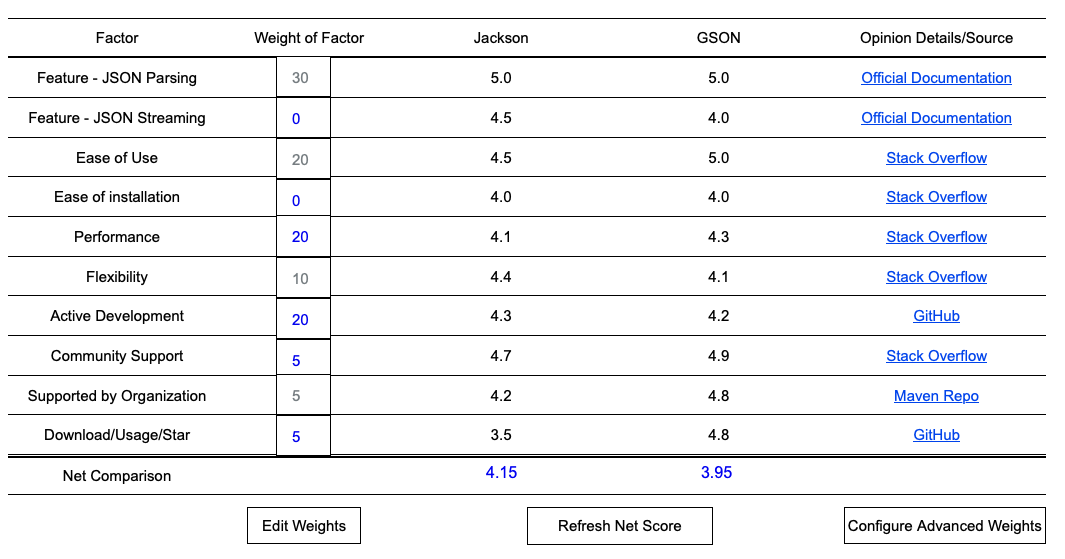
\includegraphics[scale=.25]{images/mock-ui-library-comparison.png}
%     \caption{A mock-up user interface for comparing multiple libraries along with weight of each library specific factors}
%     \label{fig:mock-ui-library-comparison}
% \end{figure}
The interviews also informed us of the feasibility of creating a tool that can help compare software libraries to support their adoption. One of our participants, a consultant with 22 years of experience, was explicit with the needs of such a tool: \qi{Let's say I would like to install a module and I would like to find third party library. I would like to have an easy way to see and I approve. I don't see any tools really for that. In many cases, I saw this: a page is trying to compare libraries but there is no objective way to compare them. Maybe there is, but there's not implemented... So that's part of the reason people don't use [libraries] because they say, OK, I don't know which one to use. This is a general problem.}{P22}

In our later interviews, we presented developers with a mock-up of such a tool, the development of which is our ongoing research. The tool design was influenced by the Fishbein Multiattribute Model \cite{fishbein1967attitude}, which aims to facilitate consumer purchase decision by assigning weights to different factors of a given product and then use the weighted averages across products to rank those. In our tool mock up UI, we thus suggested to simply assign weights to each factor (e.g, performance) of a software library. The weights would be collected from representative sources (e.g., based on user reviews on performance aspect of a library) and from a developer (e.g., the relative importance of the factor like performance over another factor like usability).
The participants who reviewed the tool during the interview also appreciated such an approach: \qi{It would be a really great tool to select some libraries because it's like our processes, we select first some keywords and afterwards, we choose a library because of our own, sometimes subjective, sometimes objective factors and here you have the right factors so you can build our process with your tool. I think we can use it in our company.}{P17}

% In addition to practitioners feedback, we also found that our library adoption model is similar to consumer and business buyer models of marketing theories \cite{kotler2014principles}. The adoption conditions in our model match with business/organization buyer behavior conditions. The two models are also similar in terms of actors. However, unlike business buying behavior model which has supplier search, selection, and performance review for traditional procurement process, the library adoption process is simpler and closely relates with the consumer buying behavior. The consumer buying process has need recognition, information search, alternative evaluation, purchase decision, and post-purchase behavior. 
% We have split the purchase decision to \code{review} (where mostly decision is taken) and \code{integrate} steps and merged \code{problem identification} under \code{search} step. Since library adoption model resembles consumer buyer behavior process, it also opens up opportunities to utilize further marketing models into library adoption process. For example, if Fishbein Multiattribute Model \cite{fishbein1967attitude} can be applied to consumer model, it can also be applied to library adoption model. Hence, if researcher propose a tool based on the weighted average of different library selection factors, developer might be able to find it useful for decision making as our participants also noted.

%The Fishbein Multiattribute Model \cite{fishbein1967attitude} can be extended to theorize library selection process through the use of marketing lens. 



% (e.g., \code{company}, \code{application domain}, \code{investment capacity}) and 15 additional selection factors (e.g., \code{ease of installation}, \code{flexibility}, \code{availability of demo}, \code{familiarity}). 
% We were further able to identify eight novel information sources such as \code{known people}, \code{search engine}, \code{existing source code}) compared with an earlier study on collecting information about open source software \cite{li2022exploring}. 

%As part of the adoption process, we have presented 5 major steps of library adoption process, identified 28 library selection factors, 14 library related source of information, and 23 internal external conditions that influence the process. No other previous study provided the process steps for libraries. Larios-Vargas et. \cite{larios2020selecting} identified 26 factors influence library selection under technical, human resource, and economical factors. Their proposed human resource and economical factors are fully mapped by our conditions category and technical factors are covered by our library selection factors. We identified 14 new conditions (such as \code{company}, \code{application domain}, \code{investment capacity}, \code{Expert/lead opinion}, \code{upgrades of OS}, \code{criticality of feature}, \code{delivery deadline}) beyond their human and economic factors. Moreover, our study also found 15 additional software selection factors (such as \code{ease of installation}, \code{flexibility}, \code{availability of demo}, \code{familiarity}, \code{used by reputed company}) which their study did not report. Besides, the factors, Li et. al outlined 14 sources for collecting information about open source software (not library) \cite{li2022exploring}. All of their reported sources are covered by our 6 information sources (\code{Package repository}, \code{Source repository}, \code{Stack Overflow}, \code{Other Q\&A sites}, \code{Online Article}, \code{Influential Blog}) and 8 of our sources are novel (such as \code{known people}, \code{search engine}, \code{existing source code}) for library information.}







\subsection{Quality and Applicability of the Study}
Corbin and Strauss did not recommend using the terms `validity' and `reliability' when discussing qualitative search \cite{corbin2014gt}, because qualitative methodologies cannot be assessed using quantitative criteria. They defined 17 measures researchers can use to evaluate the quality and applicability of their grounded theory research. We present the complete evaluation as part of our replication package \cite{website:replication-package}, here we present five major evaluation criteria.

\subsubsection{Industry Fitness}
This criterion concerns industry credibility. We conducted member checking \cite{creswell2016qualitative} by presenting a ten page summary of our findings, which was sent to 18 of our interviewees who agreed to further contact. This communication included a link to a survey which asked their opinion as to whether the summary reflected their experience and was useful to them. Thirteen participants completed the survey, all of whom opined that the summary was accurate. Five provided detailed feedback on the findings:
\qi{I think the summary captures different aspects of library selection process very well. It outlines a generic, industry-wide pattern with enough details, and also provides exceptional factors that impact that pattern.}{}

\subsubsection{Industrial Application} Industrial application answers the question of whether the findings provide insight into situations and provide knowledge which can be applied to develop policy, change practice, and add to the knowledge base of a profession \cite{corbin2014gt}. This criterion was also evaluated through member checking. One participant shared their feedback, demonstrating that they found our work applicable: \qi{One interesting thing that I learned from your research is, different developers have different processes and priorities for picking a library, and not everybody is considering all the steps that need to be taken, so I would recommend your paper to all developers to just widen their horizons.}{}

\subsubsection{Usefulness} To address this measure, we looked at if there are suggestions for practice, policy, teaching, and application \cite{corbin2014gt}. To the best of our knowledge, this is the first study to provide a comprehensive picture of library adoption. The presentation of guiding principles in the form of patterns, which are widely used in industry, makes the results more accessible to practitioners. Participants also appreciated the suggestions:
\qi{My favorite part of the summary is the takeaway action items that I believe would be useful in building a better culture for adopting the right tools and technologies.}{}

\subsubsection{Explainability of Theory} The way to assess this measure is to determine if variation is built into the theory \cite{corbin2014gt}. Our conceptual framework is based on six guiding principles which depend on different contexts and lead to different implications for the influence of conditions, factors, and use of information sources. This allows the theory to support a wide variety of circumstances.

\subsubsection{Saturation of Categories} ``How is saturation explained, and when and how was it determined that categories were saturated?'' is the criterion for evaluating this measure \cite{corbin2014gt}. We provided detailed information about how we performed theoretical sampling to achieve saturation, and described how the major categories achieved saturation throughout the progression of the study. The Appendix contains a heatmap of concept saturation which shows the progression of topics across interviews.

\subsection{Threats to Validity}
\bf{Construct validity} threats concern the relation between theory
and observations. In our study, they could arise if there is a lack of accuracy of the open coding. To mitigate this threat, two of the authors conducted the coding of several interviews separately and then discussed their codebook with each others. This approach helped us mitigate the presence of subjective bias in the coding. Threats to \bf{external validity} compromise the confidence in
stating whether the study results are applicable to other
groups. Our library adoption model is derived from the semi-structured interviews of 24 professional developers from multiple international large and small-scale software companies. We carefully adopted a theoretical sampling approach to recruit our study participants, which ensured that we collected as diverse opinions on library adoption as possible. Future studies could extend our study findings with more interviews or surveys, however, we expect that the core findings will remain.


